\documentclass[varwidth=false, border=2pt]{standalone}
\usepackage{tikz}
\usetikzlibrary{shapes}

\begin{document}
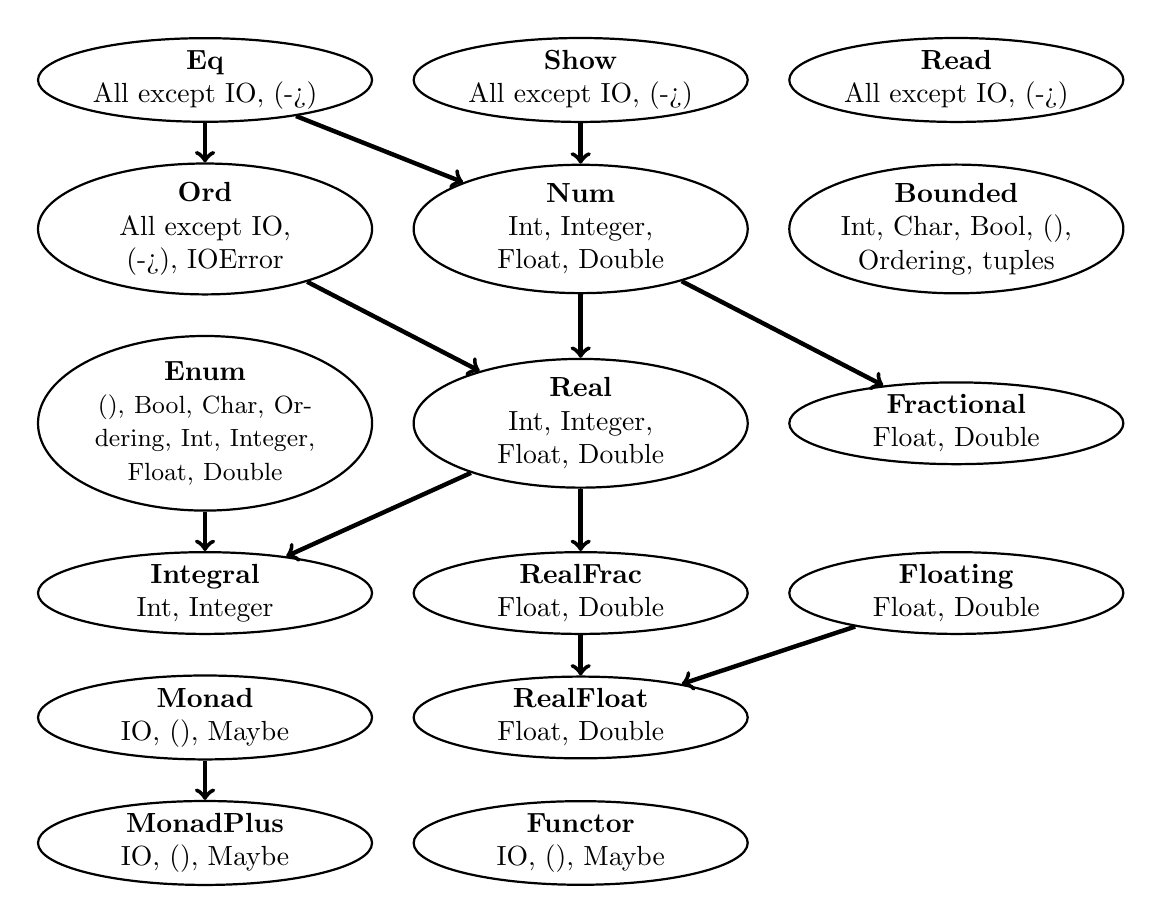
\begin{tikzpicture}
    \tikzstyle{node}=[ellipse,thick,fill=white,draw=black,inner sep=0pt,text width=3cm,align=center]
    \tikzstyle{edge}=[->, ultra thick]
    \matrix[row sep=0.5cm,column sep=0.5cm] {
    \node[node] (Eq)         {\textbf{Eq}\\All except IO, (->)};   &
    \node[node] (Show)       {\textbf{Show}\\All except IO, (->)}; &
    \node[node] (Read)       {\textbf{Read}\\All except IO, (->)}; \\
    \node[node] (Ord)        {\textbf{Ord}\\All except IO, (->), IOError};   &
    \node[node] (Num)        {\textbf{Num}\\Int, Integer, Float, Double}; &
    \node[node] (Bounded)    {\textbf{Bounded}\\Int, Char, Bool, (), Ordering, tuples}; \\
    \node[node] (Enum)       {\textbf{Enum}\\{\small (), Bool, Char, Ordering, Int, Integer, Float, Double}};   &
    \node[node] (Real)       {\textbf{Real}\\Int, Integer, Float, Double}; &
    \node[node] (Fractional) {\textbf{Fractional}\\Float, Double}; \\
    \node[node] (Integral)   {\textbf{Integral}\\Int, Integer};   &
    \node[node] (RealFrac)   {\textbf{RealFrac}\\Float, Double}; &
    \node[node] (Floating)   {\textbf{Floating}\\Float, Double}; \\
    \node[node] (Monad)      {\textbf{Monad}\\IO, (), Maybe};   &
    \node[node] (RealFloat)  {\textbf{RealFloat}\\Float, Double}; &
     \\
    \node[node] (MonadPlus)  {\textbf{MonadPlus}\\IO, (), Maybe};   &
    \node[node] (Functor)    {\textbf{Functor}\\IO, (), Maybe}; &
     \\
    };
    \draw[edge] (Eq) -- (Ord);
    \draw[edge] (Eq) -- (Num);
    \draw[edge] (Show) -- (Num);
    \draw[edge] (Ord) -- (Real);
    \draw[edge] (Num) -- (Real);
    \draw[edge] (Num) -- (Fractional);
    \draw[edge] (Enum) -- (Integral);
    \draw[edge] (Real) -- (Integral);
    \draw[edge] (Real) -- (RealFrac);
    \draw[edge] (Floating) -- (RealFloat);
    \draw[edge] (RealFrac) -- (RealFloat);
    \draw[edge] (Monad) -- (MonadPlus);
\end{tikzpicture}
\end{document}
